\documentclass[12pt,a4paper,openright,twoside]{book}
\usepackage[utf8]{inputenc}
\usepackage{disi-thesis}
\usepackage{code-lstlistings}
\usepackage{notes}
\usepackage{shortcuts}
\usepackage{acronym}

\school{\unibo}
\programme{Corso di Laurea [Magistralfe?] in Ingegneria e Scienze Informatiche}
\title{Fancy Title}
\author{Candidate Name}
\date{\today}
\subject{Supervisor's course name}
\supervisor{Prof. Supervisor Here}
\cosupervisor{Dott. CoSupervisor 1}
\morecosupervisor{Dott. CoSupervisor 2}
\session{I}
\academicyear{2022-2023}

% Definition of acronyms
\acrodef{IoT}{Internet of Thing}
\acrodef{vm}[VM]{Virtual Machine}


\mainlinespacing{1.241} % line spacing in mainmatter, comment to default (1)

\begin{document}

\frontmatter\frontispiece

\begin{abstract}	
Max 2000 characters, strict.
\end{abstract}

\begin{dedication} % this is optional
Optional. Max a few lines.
\end{dedication}

%----------------------------------------------------------------------------------------
\tableofcontents   
\listoffigures     % (optional) comment if empty
\lstlistoflistings % (optional) comment if empty
%----------------------------------------------------------------------------------------

\mainmatter

%----------------------------------------------------------------------------------------
\chapter{Introduction}
\label{chap:introduction}
%----------------------------------------------------------------------------------------

Write your intro here.
\sidenote{Add sidenotes in this way. They are named after the author of the thesis}

You can use acronyms that your defined previously,
such as \ac{IoT}.
%
If you use acronyms twice,
they will be written in full only once
(indeed, you can mention the \ac{IoT} now without it being fully explained).
%
In some cases, you may need a plural form of the acronym.
%
For instance,
that you are discussing \acp{vm},
you may need both \ac{vm} and \acp{vm}.

\paragraph{Structure of the Thesis}

\note{At the end, describe the structure of the paper}

\chapter{State of the art}

I suggest referencing stuff as follows: \cref{fig:random-image} or \Cref{fig:random-image}

\begin{figure}
    \centering
    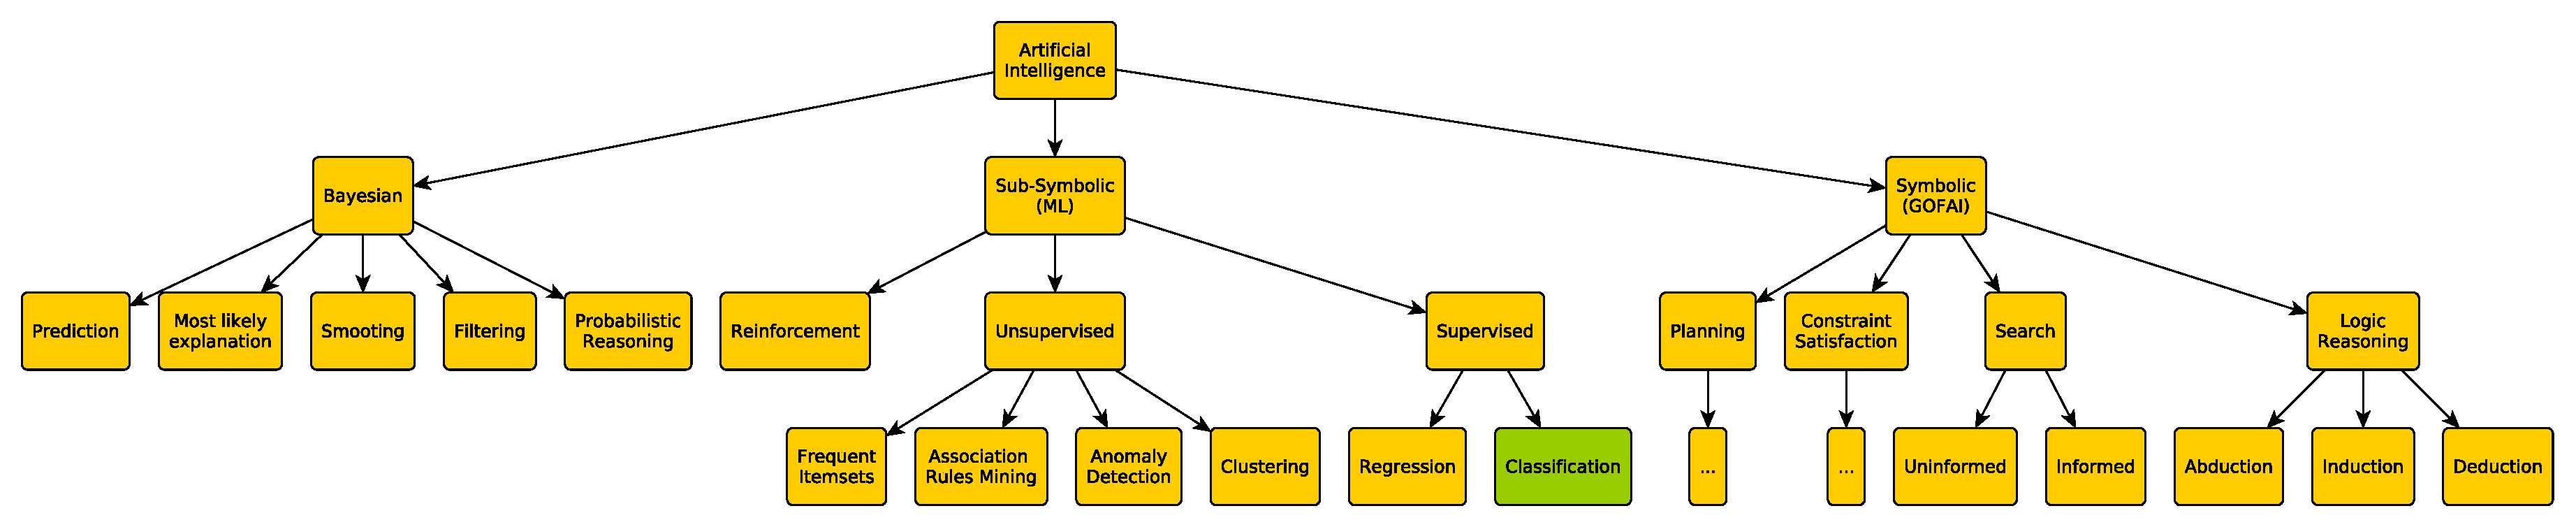
\includegraphics[width=.8\linewidth]{figures/random-image.pdf}
    \caption{Some random image}
    \label{fig:random-image}
\end{figure}

\section{Some cool topic}

\chapter{Contribution}

You may also put some code snippet (which is NOT float by default), eg: \cref{lst:random-code}.

\lstinputlisting[float,language=Java,label={lst:random-code}]{listings/HelloWorld.java}

\section{Fancy formulas here}

%----------------------------------------------------------------------------------------
% BIBLIOGRAPHY
%----------------------------------------------------------------------------------------

\backmatter

\nocite{*} % Remove this as soon as you have the first citation

\bibliographystyle{alpha}
\bibliography{bibliography}

\begin{acknowledgements} % this is optional
Optional. Max 1 page.
\end{acknowledgements}

\end{document}